\documentclass{beamer}

\newcommand{\darkLogo}{$\vcenter{
\includegraphics{tallogo-dark.pdf}}$}
\usepackage{wrapfig}
\usefonttheme{serif}
\usepackage[no-math]{fontspec}
\usepackage{amsmath,amsfonts,amssymb,stmaryrd}

\def\yo{\text{y}}
\def\pto{\rightsquigarrow}
\def\Prof{\textbf{Prof}}
\def\Lan{\text{Lan}}

\definecolor{bleakYellow}{HTML}{F0DB4F}
\setmainfont{Source Sans Pro}

\usetheme[background=dark]{metropolis}
\setbeamercolor{alerted text}{fg=bleakYellow}

\setbeamertemplate{footline}{}

\author{Fosco Loregian \darkLogo}
\title{}
\date{\today}

\setbeamertemplate{navigation symbols}{}

\usepackage[all,2cell]{xy}\UseAllTwocells

\begin{document}
\begin{frame}
  \maketitle
%   \centering
%   \Huge FOSCO LOREGIAN \\
\end{frame}
\begin{frame}
  \begin{itemize}
    \item<+-> Ph.D. at SISSA - Trieste 
\includegraphics{ita.pdf}

    \indent {\footnotesize Stable homotopy theory, ∞-categories, derived AG}
    \item<+-> University of Western Ontario 
\includegraphics[scale=.04]{can.pdf}
    
    \indent {\footnotesize ∞-categories, derivators}
    \item<+-> Masaryk University 
\includegraphics{czr.pdf}
    
    \indent {\footnotesize Accessible categories, derivators, 2-categories}
    \item<+-> Max Planck Inst. für Math. 
\includegraphics{ger.pdf}
    
    \indent {\footnotesize 2-categories, derivators, applied category theory}
    \item<+-> Centro de Matemàtica da Universidade de Coimbra 
\includegraphics[scale=.04]{por.pdf}
    
    \indent {\footnotesize 2-categories; finishing my first book}
    \item<+-> Tallinna Tehnikaülikooli 
\includegraphics{est.pdf}
    
    \indent {\footnotesize 2-categories; functorial semantics; categorical probability theory and its applications}
  \end{itemize}
\end{frame}
%
%
%
%
%
\begin{frame}
  \Huge\centering \bfseries STABLE HOMOTOPY THEORY
\end{frame}
%
\begin{frame}
  \alert{∞-categories}: a thickening of the notion of category, suitable for homotopy-invariant mathematics (algebraic geometry, algebraic topology type theory).
  
  \onslide<+->
  Turns out some parts of Mathematics are easier if stated in these terms:
  \begin{itemize}
    \item homological algebra : the scary part of algebraic topology 
    
    {\footnotesize higher algebra: the linear algebra of ∞-categories}
    \item 1-topos theory : a synthetic type theory,
    
    {\footnotesize ∞-topos theory: a synthetic homotopy theory of homotopy types}
  \end{itemize}
\end{frame}
%
%
%
%
%
\begin{frame}
  A stable ∞-category is an ∞-category
\begin{itemize}
\item with all finite limits and colimits
\item such that a square is cartesian iff cocartesian
\end{itemize}
\onslide<+->
The homotopy category of a stable ∞-cat is always triangulated.

\onslide<+->
The correspondence sending an abelian category $\cal A$ into its derived category has a nice and clear universal property stated in terms of the heart of a canonical $t$-structure.

\onslide<+->
Stable, rational, p-adic, ...  homotopy theory become pieces of the commutative algebra of  ∞-categories
\end{frame}
%
%
%
%
%
\begin{frame}
  A t-structure on a triangulated $\cal D$ is a pair of triangulated subcategories of D such that every object X lies in a sequence
\[X_{\le} \to X \to X_\ge \to X_\le[1]\]
[\alert{FL14}] : On stable ∞-categories a t-structure is a factorization system (E,M)
\begin{itemize}
\item<+-> such that E and M are 3-for-2 classes
\item<+-> thus the category of E-cofibrant objects is coreflective
\item<+-> and the category of M-fibrant objects is reflective
\item<+-> cof/fib replacement = neg/pos truncation
\end{itemize}
\onslide<5->
(Algebraic) geometry reduces to a piece of categorical algebra.
\end{frame}
%
%
%
\begin{frame}{Plan: redo $t$-structures}
  \begin{itemize}
\item<+-> {} [\alert{FL15}] The set of t-structures has a natural choice of $\mathbb Z$-action ($\mathbb Z$ = the integers); so, study $\mathbb Z$-equivariant monotone maps from a poset J to TS(C).

{\footnotesize This describes Bridgeland stability manifolds, and Postnikov towers on ∞-toposes.}

\item<+-> {} [\alert{FL15b}] Every stratified manifold $(X,\mathfrak s)$ generates a pair of t-structure that can be glued together

{\footnotesize recollements, stratified schemes, representation of algebras}

  \end{itemize}
\end{frame}
%
%
%
%
%
\begin{frame}{Plan: redo $t$-structures}\small %{Every PhD finishes with two conjectures\dots}
  %  In [\alert{FL?}, work in progress] Rational and $p$-adic homotopy ~ rational and $p$-adic geometry ~ ``number-theoretic'' factorization systems:

   \begin{itemize}
     \item<+-> The space of \alert{slicings} on a stable ∞-category is a metric space and
     
     \item<+-> The space \[\{ J \colon \mathbb R \to TS(\mathcal C) \mid J \text{ is Sorgenfrey continuous} \}\] 
     is an interesting set [\alert{L-PhD}]
    \end{itemize}

    \onslide<+->
    \begin{block}{Conjecture}
  Study
\[\{ J \colon \text{Spec}(\mathbb Z) \to TS(\mathcal C) \mid J \text{ is Zariski continuous} \}\]
to get something about motivic t-structure.
 \end{block}
 \onslide<+->
 \begin{block}{Conjecture}
 Blakers-Massey in positive characteristic is a theorem about factorization systems.
 \end{block}
\end{frame}
%
%
%
%
\begin{frame}{Morse theory as a theory of FS}
  \begin{wrapfigure}[5]{l}{.5\textwidth}
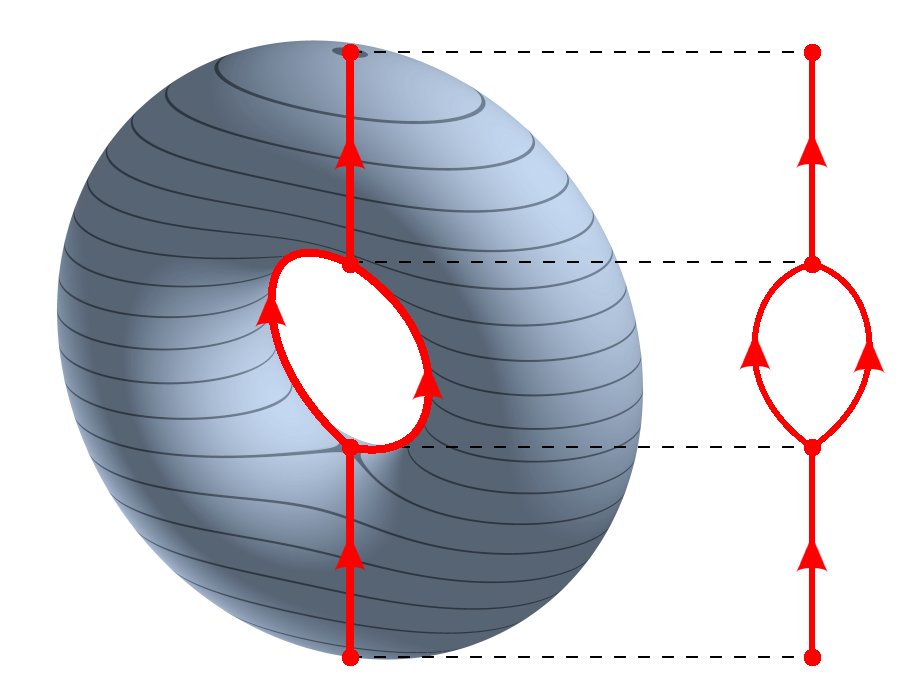
\includegraphics[scale=.15]{3D-Leveltorus-Reebgraph.png}
  \end{wrapfigure}
  
  Fact: Bord(n) is the free (∞,n)-symmoncat on the point.
  
  \vspace{1cm}
  Monoidal functors $Z : Bord(n) \to Vect$ are completely classified.

  \vspace{1cm}
  \onslide<+->
  Morse theory is the theory of suitable factorization systems on Bord(n).

  \alert{critical points of a Morse function}
  correspond to

 \alert{critical values} [\alert{L-PhD}, Ch.7] of a certain slicing $J : \mathbb R \to FS(Bord(n))$.
\end{frame}
%
%
%
%
%
%
%
\begin{frame}
  \Huge\centering \bfseries DERIVATORS
\end{frame}
%
\begin{frame}
  A derivator is a strict 2-functor
  \[\mathbb{D} : {\bf Cat}^\text{op} \to {\bf CAT} \]
  satisfying stacky conditions. They form the 2-category Der.

  They subsume most of ∞-category theory; in particular, their stable homotopy.
  \begin{itemize}
    \item<2-> [{[\alert{LV17}]}] : A t-structure on a stable derivator is still a certain kind of factorization system; FS are still strict 2-algebras for the "squaring" 2-monad ( \_ )² : A mapsto A² (see [\emph{KT93}])
    
    \item<3->  [{[\alert{Lor18}]}] : reflective subderivators correspond to reflective factorization systems, and to algebras for idempotent monads

    (the "formal theory of monads" [\emph{S80}] still holds in Der, a monad $T : D \to D$ is just defined objectwise)
  \end{itemize}
\end{frame}
%
\begin{frame}
  There is a \alert{Yoneda structure}\footnote{A 2-categorical device to encode the calculus of pointwise Kan extensions.} on the 2-category of derivators

  If this is true
\begin{itemize}
\item<2-> comprehensive account of various notions of \alert{accessible} and \alert{locally presentable} derivator using the theory of locally presentable objects in a Yoneda structure, done in [\alert{DLL18}]; categorical logic for derivators (see Prest's treatment of \alert{definability} for module categories); derivator topos theory?
\item<3-> a convincing form of \alert{adjoint functor theorem} for derivators; existence of a six-operation calculus for mappings of derivators. 2-categorical account of Grothendieck duality complicated diagrams...
\item<4-> \alert{profunctors} between derivators; fibered derivators; \alert{operads} in derivator theory; applications in representation theory of algebras, stable homotopy, ...
\end{itemize}
\end{frame}
%
%
%
%
%
%
\begin{frame}
  \Huge\centering \bfseries COENDS AND DG-STUFF
\end{frame}
%
\begin{frame}
  I have written a book on \alert{coend calculus}, soon to appear under Cambridge University Press LNMs:
\begin{wrapfigure}{l}{.35\textwidth}
  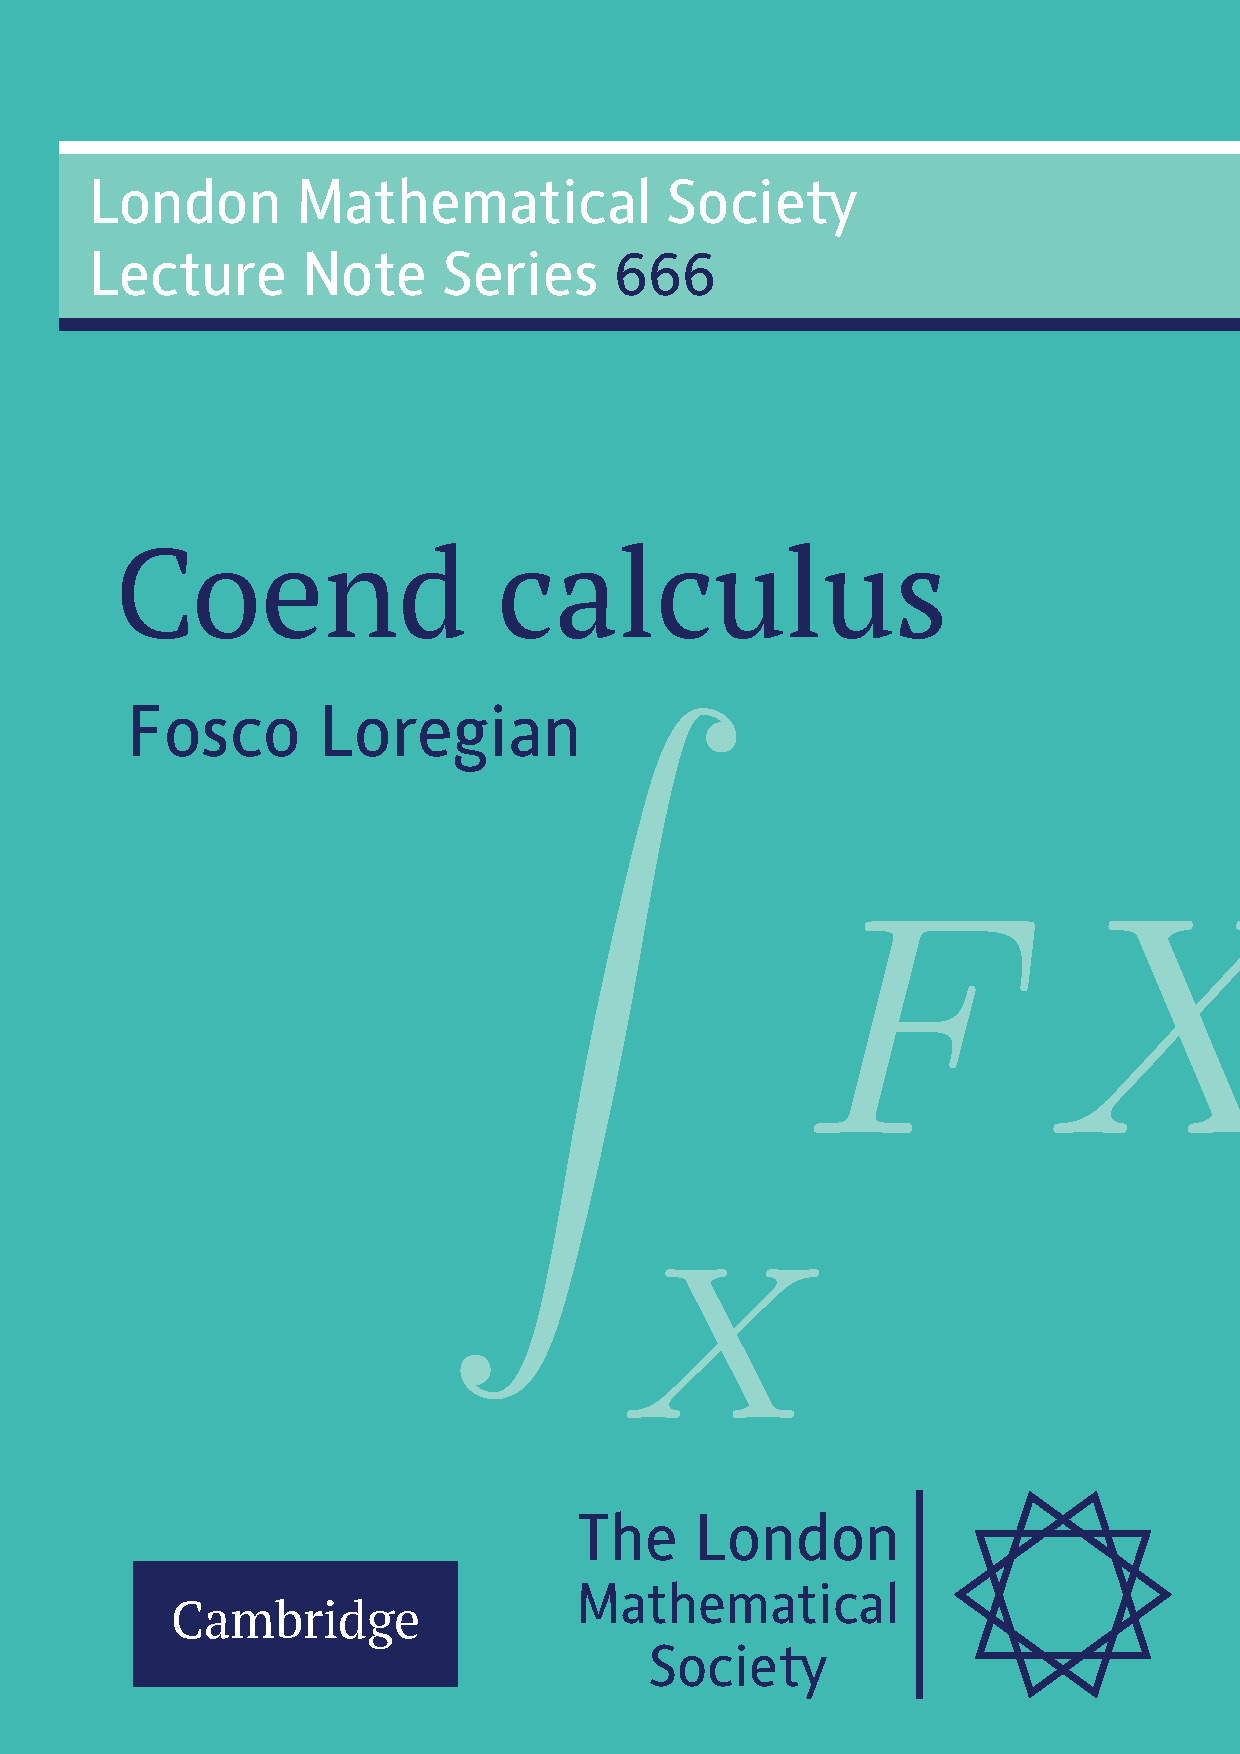
\includegraphics[width=.35\textwidth]{cover-2-.pdf}
\end{wrapfigure}
\small
\begin{itemize}
  \item<+-> Coends $\int_C T$ are universal objects associated to $T : C^{op}\times C \to D$, treated as integrals (a ``Fubini rule'' is valid).
  \item<+-> They find application in (monoidal) category theory, algebraic topology, algebraic geometry, categorical logic, representation theory (see ch.7 for an application to \alert{DG-categories}), functional programming\dots
  \item<+-> The book is being extensively cited (45 citations on Scholar \today)
\end{itemize}
\end{frame}
%
%
%
%
\begin{frame}
  In [\alert{L20}, 7.2.2]
  \begin{center}
  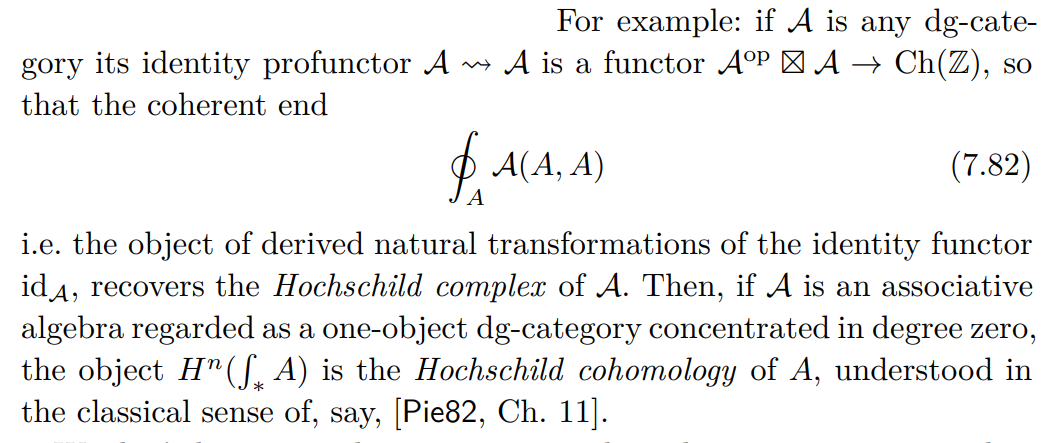
\includegraphics[width=.75\textwidth]{dg.png}
  \end{center}
  \onslide<2->
  Applications to Kuznetsov-Lunts \alert{categorical resolutions of singularities}: a smooth DG-category is a $\cal D$ such that its identity profunctor $h : {\cal D} \rightsquigarrow \cal D$ is a perfect object (read as: a variety is smooth if the diagonal map $\Delta : X \to X\times X$ is smooth)
\end{frame}
%
%
%
%
%
\begin{frame}
  \Huge\centering \bfseries TEACHING AND ORGANIZATIONAL ACTIVITIES
\end{frame}
%
\begin{frame}\small
  \begin{itemize}
    \item<+-> 2015 A short course on \alert{model categories} at the University of Pavia
    \item<+-> 2015 and 2019 Attendee and speaker at the \alert{Kan Seminar I} (a webinar on category theory), and \alert{Applied Category Theory} 2019 (a webinar on applied category theory, from which the paper [\alert{MLR$^{+}$20}] stemmed)
    \item<+-> 2016 ``\alert{Elements of Finite Mathematics}'' at UWO (mostly statistics to kinesiologists)
    \item<+-> 2016 \alert{Advisor} of a BSc thesis @unibo, "Elementary aspects of adjoint functors" 
    \item<+-> 2018 \alert{Organiser} of the 103rd Peripathetic Seminar on Sheaves and Logic, Brno
    \item<+-> 2020 \alert{Category theory} course Teacher @taltech
    \item<+-> 2019 and 2020 \alert{Organiser} of ItaCa (\alert{Ita}lian \alert{Ca}tegory theorists) in Milan and on zoom, due to COVID19.
    \item<+-> Reviewer for zbMath and AMS.
  \end{itemize}
\end{frame}
%
%
%
%
%
%
%
\begin{frame}{Miscellaneous projects}
\small 
\begin{itemize}
  \item<+-> Homotopy theory and set theory: [\alert{DL18}] no homotopy category of a model category is ``concrete''; what about $\infty$-categories?
  \item<+-> Functional programming and type theory: HoTT, linear types, proof-checkers, categorical algebra in relational database architecture; natural language processing using category theory\dots
  \item<+-> Categorical logic and foundations of mathematics; functorial semantics à la Lawvere, but sprinkled with operads
  \item<+-> more in detail, ``2-semantics'' of algebraic theories: profunctorial PROPs and theories, categorical algebra of cartesian bicategories\dots
\end{itemize}
\end{frame}
%
\begin{frame}
  
\end{frame}
%
%
%
%
%
\end{document}